


\documentclass[main]{subfiles}

\begin{document}

\chapter{Related Work}

\section{Scope of Research} \label{sec:scoperesearch}

In Chapter 1 (``Approaches to Interpretability'') a brief overview of feature attribution methods was provided with reference to a distinction between model-specific and model-agnostic methods. This is a common distinction in the literature and was also used to guide research in this project. The panel of methods chosen for evaluation ultimately consisted of a balanced selection from both approaches. 

A major difficulty of this project was distilling the broad literature on these methods however. For the model-specific (neural network) family, different angles are commonly taken to calculate feature ``relevance'' or importance. These include generally:
\begin{itemize}
\item \textbf{Backpropagation-based} methods or `importance signal' projections (such as activations in a hidden layer)
\item \textbf{Gradient-based} methods, saliency maps and output sensitivity methods
\item \textbf{Perturbation-based} methods and input occlusion techniques
\end{itemize}

This categorisation is based on two recent papers that make similar categorisations of explanation approaches  \cite{deeplift} \cite{patternnet}. In this chapter a broad selection of methods based on traction over time, current popularity and representativeness of approach are described, though the reader should note there are more methods under each of those three than have been described here.

For model-agnostic methods, perturbation-based and other miscellaneous approaches are considered. Again the selection was based on traction and literature popularity.

First reviewed are traditional, visual approaches to interpretability to provide context to the task of feature attribution. After the exploration of feature attribution methods, a review of existing evaluation metrics and comparison studies is provided.

\subsection*{Terminology}
All methods are variously referred to as \textit{attribution} methods in this project for any projection on the input space that highlights relevant features. Adebayo et al. (2018) instead refer to the broad category of ``[...] visualisation and attribution methods aimed at interpreting trained models'' as \textit{saliency} methods, particularly in the context of image data \cite{sanity}. Including by those authors, a \textit{saliency map} is widely used as a catch-all term to refer to input space projections (individual explanations) in the context of interpreting deep neural networks for image data. However they also refer to a specific gradient-based method (Section \ref{sec:gradient}). 

Consensus on terminology is relatively lacking. Some researchers (\cite{patternnet}) describe attribution methods as a subclass of explanation techniques where contribution scores are specifically calculated for each input feature (i.e. excluding higher level `patterns' which cause neuron activations, as in Zeiler \& Fergus (2013) (\cite{zeilerfergus2013}), (Section \textbf{X}) or the back-propagation class generally). 

In summary, attribution methods is used in this report as a general term for explanation methods. Saliency maps, explanations and attributions are all interchangeably used for any attribution method's output.

% also sensitivity map or pixel attribution map as by SmoothGrad

\section{Traditional Approaches}

\subsection{Feature Projection}
Visualisation tools for high-dimensional data are a popular way to gauge insight into expected model behaviour.  These pre-learning, exploratory data analysis techniques include mathematical reductions like PCA and probabilistic techniques like t-SNE,  projecting high-dimensional examples that are `similar' into a visualisable 2D or 3D space \cite{tsnepaper} (Figure \ref{tsneimg}).

\begin{figure}[h]
\centering
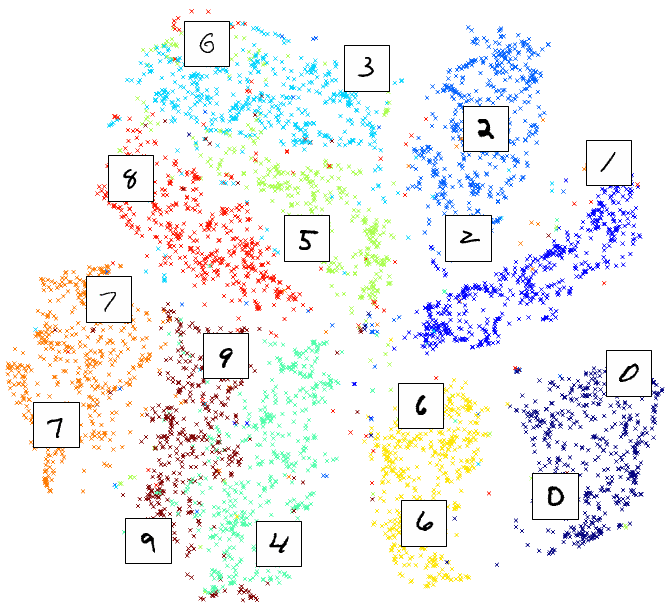
\includegraphics[scale=0.2]{tsne.png}
\caption{2D embedding of 70,000 handwritten digits (0-9) from MNIST \cite{tsne}.}
\label{tsneimg}
\end{figure}

Other methods of clustering and dimensionality reduction are also widely used for interpreting data, and although useful for gaining an intuition on relationships between features, they are not suited for explaining model behaviour as they examine only the input space itself. 

\subsection{Partial Dependence Plots}

A partial dependence plot (PDP) is a tool to demonstrate the marginal effect of one or two features on a prediction outcome. It was proposed by Friedman in 2001 to interpret and visualise the features that the proposed gradient boosting machine relied upon (though it is limited to 1 or 2 input features such that it can be displayed) \cite{pdp1}. A partial dependence function $\widehat{f_{xs}}$ can be calculated for some desired set of features S, by marginalising the model output over the set of `complement` features C (all other features):
\begin{align}
\widehat{f_{xs}}=\int \widehat{f}(x_{s}, x_{c})dP(x_{c})
\end{align}
It can be approximated with a Monte Carlo method. Friedman believed in 2001 that these might be used to help interpret ``any black box prediction method'' such as NN and SVM architectures, and that, ``[...] when there are a large number of predictor variables, it is very useful to have a measure of relevance to reduce the potentially large number of variables to be considered" \cite{pdp1}. The mentioned relevance measure was defined only in the context of the decision trees which constituted the paper's gradient boosting machine. Certainly, PDPs are suited for the low-dimensional feature spaces that were imagined in the pre-deep learning era, and are less suitable for high-dimensional input spaces such as in image classification. They are also restricted by an unrealistic assumption of independence among features.

\section{Model-Specific Methods} \label{sec:modelspec}
Deep learning's reputation for lack of transparency has led to many attempts to explain the predictions of complex NN architectures. This section examines representative attribution methods from the backpropagation-based, gradient-based and perturbation-based approaches overviewed in Section \ref{sec:scoperesearch}, with some emphasis on those developed in the context of CNNs (i.e. image data).


\subsection{Backpropagation-Based} \label{sec:backprop}

Methods in this class try to isolate an internal model signal, such as neuron activations in a target hidden layer, and map these signals back into the input pixel space. Zeiler \& Fergus (2013) introduced the motivation for signal backpropagation as ``[...] showing what input pattern originally caused a given activation in the feature maps'' \cite{zeilerfergus2013}. 

\subsubsection{Visualising Activations - DeconvNet, Guided Backpropagation}
Visualisation of per-layer activations is one approach to explain inner model behaviour. It is different from other feature attribution approaches in that it seeks to visualise `learned features' instead of the contributions of input space features. DeconvNet and Guided Backpropagation are two popular examples of the approach and are briefly described as two forerunners of the backpropagation (and gradient) approach.

Deconvolutional networks (DeconvNet) generate backwards projections of neuron activations, by reversing individual activations during a `deconvolution' backwards-pass \cite{zeilerfergus2013}. The procedure can be summarised as passing feature map output activations as input into `deconv' layers, iteratively reversing activations and reconstructing input signals until the input pixel space is reached.

\begin{figure}[h]
\centering
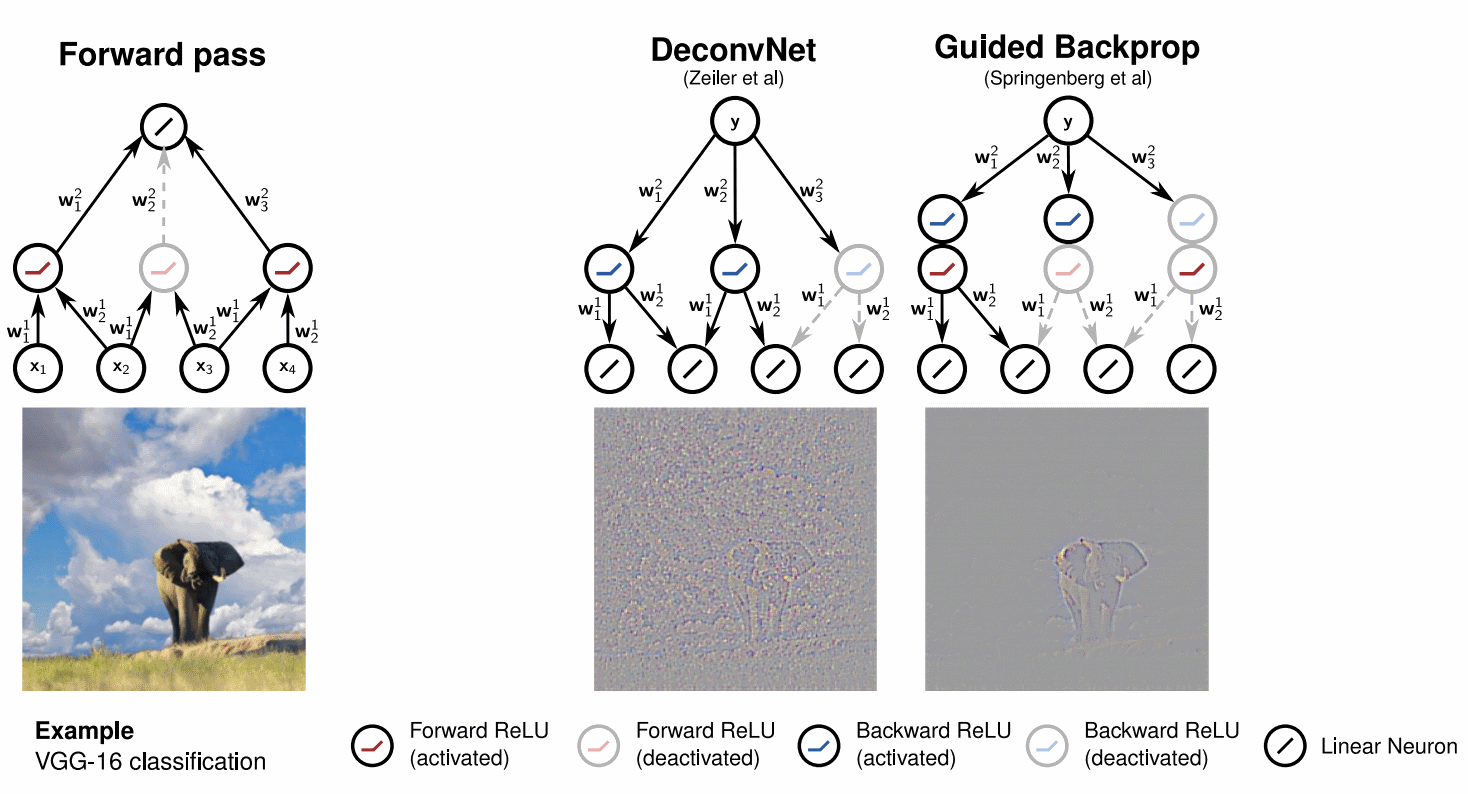
\includegraphics[scale=0.3]{deconv.png}
\caption{(Adapted from \cite{patternnet}) Illustration of DeconvNet and Guided Backprop.}
\label{deconvimg}
\end{figure}

Since it can target one layer's activation at a time, the method is useful for understanding the hierarchical learned features that CNNs generate over multiple layers. Its limitation is that during the backwards pass, it ignores any negative inputs to ReLu activations that were zero'd out in the forward pass (deactivated activations in Figure \ref{deconvimg}).

Guided Backpropagation was an enhancement by Sprigenberg et al. (2014) that added an additional signal at each step by zero'ing the importance signal if it was a negative activation in the forward pass phase \textit{or} negative in the backwards pass (the two intermediate signals in Figure \ref{deconvimg} right) \cite{springenberg}. This stopped negative gradients in lower layers from decreasing the activation of the higher layer units which were the target, and this leads to sharper explanations than those created by DeconvNet \cite{springenberg}. 

\subsubsection{DeepLIFT}

DeepLIFT (Deep Learning of Important FeaTures) \cite{deeplift} was created out of the motivation that the zero'ing of negative gradients by DeconvNet and Guided Backpropagation meant that neither are able to highlight inputs that contribute negatively to an output. In some sense they are therefore missing half the story of feature contribution / neuron activation. DeepLIFT's authors (Shrikumar et al. (2017)) also wanted to overcome the unaddressed saturation problem, which is that relevant neurons that contribute to a saturated output activation would not individually change the output if they were turned off (as might be tried in perturbation approaches).

DeepLIFT's innovation over previous backpropagation and gradient-based methods was to realise that where this problem existed, a single gradient value of an output with respect to an input value did not adequately or necessarily capture input contributions to an output. The authors' proposal was to find input contributions by instead calculating the absolute change in output with respect to a neuron's `reference' activation. 

\begin{figure}[h]
\centering
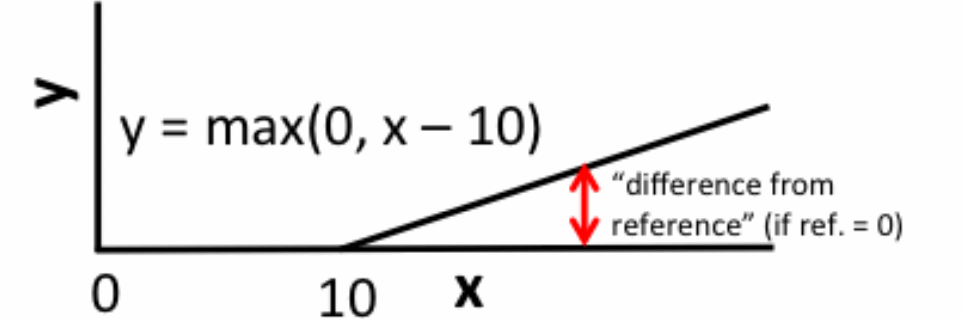
\includegraphics[scale=0.3]{deeplift.png}
\caption{(From \cite{deeplift}) Difference-from-reference attributions can avoid bias terms.}
\label{deepliftimg}
\end{figure}

Finding reference activations is an implementation difficulty. Generally, the authors propose all-zero input as a baseline (a black square for image data), and a better reference to be the average input over a background data sample \cite{deeplift}.

Like other backpropagation methods, DeepLIFT is extremely fast to calculate as it requires only a single backwards pass to propagate an importance signal back into the input space. The authors also provide different formulations for practical implementation, and a relatively high-level public implementation \cite{deepliftrepo}. The concept itself is also compatible with any NN architecture or application, unlike for example DeconvNets and Guided Backpropagation, designed for ReLu activation functions, and GradCAM (Section \textbf{X}) which was designed for CNNs.


\subsubsection{Other Backpropagation Methods}
DeepLIFT is one of several modern methods to decompose a network's prediction onto input features using activation backpropagation. For brevity its main competitors, Layerwise Relevance Propagation \cite{lrp} and DeepTaylorDecomposition \cite{taylor}, are omitted here but mentioned for the reader's reference.


\subsection{Gradient-Based} \label{sec:gradient}
These methods aim to explain a class output in terms of sensitivity in the input space by relying on a gradient function of the output\footnote{There is a strong overlap between gradient and backprop. methods: gradients as derivatives are approximated via backprop, and the weights updated by these gradients in training are the contributions to the neuron activations measured via backprop. techniques.}. The goal is to find the input features that make that prediction more or less confident: for example, for an output class of `tree' they seek to answer ``what makes a tree more/less a tree?''.

\subsubsection{Saliency Maps}
An early formulation of a local explanation method was provided by Baehrens et al. (2010) for any nonlinear classification algorithm (though developed in the context of Bayesian classification) \cite{saliencyI}. The local explanation gradient vectors that this paper devised were based on class probability gradients, characterising how much a data point has to be moved for a predicted label to change.

Simonyan et al. (2014) later applied a similar idea to CNNs to create `class saliency maps' specific to a given image and class \cite{saliencyII}. 

\begin{figure}[h]
\centering
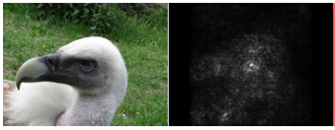
\includegraphics[scale=0.8]{saliency.png}
\caption{(From \cite{saliencyII}) Example of an image-specific class saliency map.}
\label{saliencyimg}
\end{figure}

The formulation is based on finding the derivative of an output class with respect to an input image via back-propagation. The authors also formulate a method to generate an image that maximises the output class score for a particular class, to visualise the model's `interpretation' of a class. 

%The method of computing gradients of DeconvNet-based reconstruction of the input to a hidden layer (Section 1.3.1) is equivalent to computing the gradient of visualised neuron activations with respect to that input \cite{saliencyII}.


This paper sparked great interest in CNN explanations and further interest in creating explanations from network gradients generally. Along with DeconvNet and Guided Backpropagation (developed relatively simultaneously with similar ideas) these three methods are the most historically popular and influential saliency techniques\footnote{Saliency maps are synonymous with gradient methods to the point where it is sometimes referred to as simply the `Gradients' technique, as in Adebayo et al. (2018) \cite{sanity}, who may have done so to disambiguate the technique from saliency maps generally - see Section 1.1 (``Terminology'').}. A drawback of saliency maps is that noisy images can be produced when a model does not distinguish between objects that are being predicted and nearby objects that are associated (i.e. a tree with leaves, in an image of a bird).

\subsubsection{Grad-CAM}
Class activation maps (CAMs) are another approach aimed at understanding the behaviour of CNNs introduced by Zhou et al. (2015) \cite{cam}, based on the motivation that deeper convolutional layers capture higher-level visual constructs while retaining spatial information \cite{gradcam}. While examining global average pooling (GAP) layers, a technique previously suggested for regularisation during training \cite{nin}, the authors realised a final convolutional layer's separate RGB channels (or `feature maps') could be input into a GAP layer with outputs used as features in a fully-connected layer, just before the final softmax layer. The class-associated weights in that fully-connected layer can be combined with the original final convolutional layer feature maps to capture deep representations as object localisations/class `activation' maps:

\begin{figure}[h]
\centering
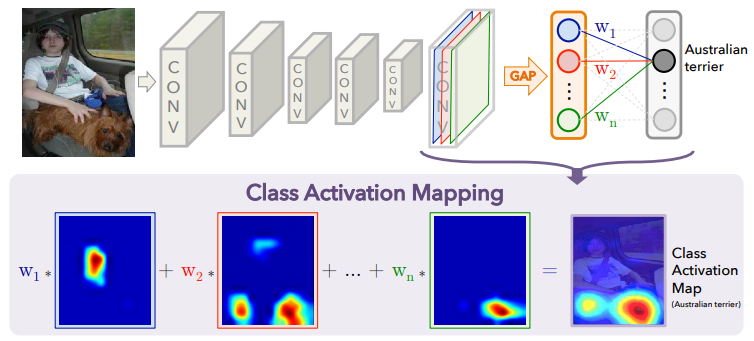
\includegraphics[scale=0.5]{cam.png}
\caption{(From \cite{cam}) Summary of the CAM formulation. RGB channels are emphasised as inputs into the weighted sum that creates a CAM.}
\label{camimg}
\end{figure}

A major limitation of the CAM approach is that it requires specific CNN architectures without previous fully-connected layers, and a GAP layer to be added before the output softmax layer to generate the deep representations it visualises. As well as this being a hurdle to adoption, the representations are highly coarse and only roughly approximate class-associated regions (a reason for heatmap presentation).

Grad-CAM was proposed by Selvaraju et al. (2016) aimed at making CAMs applicable to a wider range of CNN models, and for visual tasks other than image classification \cite{gradcam}. It requires no alteration to model architecture. It still targets the final convolutional layer's channels, as in CAM, but uses the \textit{gradient} of an output class score with respect to these channels' output activations to then globally-average-pool the gradients over the layer's width and height dimensions. The importance weights produced can be visualised as a localised heatmap over the input space, though the authors also multiply a Guided Backpropagation output (Section \ref{sec:backprop}) with the heatmaps to generate a class-discriminative, ``high-resolution'' version called Guided Grad-CAM (Figure \ref{gradimg}).

\begin{figure}[h]
\centering
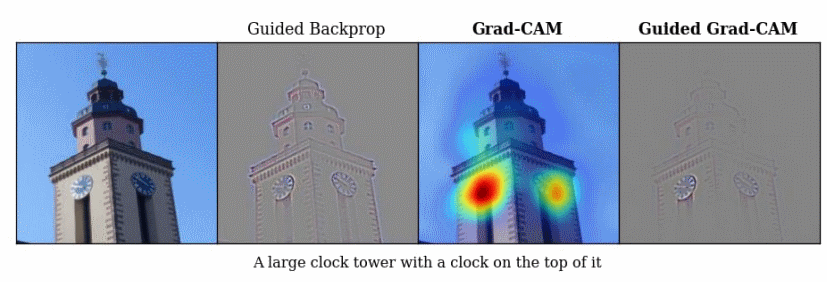
\includegraphics[scale=0.6]{gradcam_I.png}
\caption{(Adapted from \cite{gradcam}) \textit{Guided Backpropagation}, \textit{Grad-CAM} and \textit{Guided Grad-CAM} on an image captioning example from the Neuraltalk2 model.}
\label{gradimg}
\end{figure}

One of Grad-CAM's strengths is that its authors prove its effectiveness for a variety of use cases. These include highlighting causes of incorrect predictions (`failure modes'), the effect of adversarial noise and causes of model confusion, and identifying training dataset bias\footnote{For example, they showed that a VGG model trained to classify nurses from doctors had learned to look at long hair to incorrectly label a female doctor a nurse, and the bias was because of gender-skewed training data.}. Its application to a variety of models by other researchers (\cite{gradcamplusplus}, \cite{xray}) is one testament to its authors' claims on cross-model applicability and explanation quality, as well as its popularity in the literature ($>$2000 citations). 

%gradcam efficient variation https://arxiv.org/abs/1911.11293
% gradCAM has over 2000 citations
%Occlusions for Effective Data Augmentation in Image Classification
%https://arxiv.org/abs/1910.10651
% gradCAM was also used by the introduction motivating example


\subsubsection{Other Gradient Methods}

Three other gradient-based methods are widely cited and relevant to discussion - Integrated Gradients \cite{integrated}, Gradient * Input \cite{olddeeplift} and SmoothGrad \cite{smoothgrad}. 

Integrated Gradients is similar to DeepLIFT - instead of taking difference-from-reference activation as a signal of contribution, the approach is to integrate the possible gradients over all inputs (from 0 up to the activation caused by the input image) and then use this area under the activation function as an information measure of input relevance. It also addresses the saturation problem (Section \ref{sec:backprop}) though is naturally expensive to compute. Approximating the integral requires a baseline example that can provide zero input score as a comparison, and the method is applicable to a variety of architectures (two other similarities with DeepLIFT).

Gradient * Input was a simple proposal by DeepLIFT's authors to sharpen the saliency maps of Simonyan et al. (2014) \cite{saliencyII} by multiplying the gradient with the original input signal. SmoothGrad was another attempt to sharpen gradient-based saliency maps, that noted gradients as derivatives can fluctuate sharply at local scales. To compensate for the noise in the output explanation, they propose a local average of gradient values that can be computed based on random samples of the original input image with Gaussian noise added.

%<put figure in comparing gradient and backprop ones i.e. deep %explainer or patternattribution>

\subsection{Other Model-Specific Techniques} \label{sec:otherms}

Backpropagation and gradient methods can be viewed as reflections of one approach based on a similar assumption: that propagating a relevant signal back through a neural network model is a means to explain how the signal was originally encoded. A third and more unrelated category of model-specific methods are perturbation techniques. These treat the underlying model as a true black-box by iteratively occluding patches of the input feature space in order to measure the change in output class score. Where the occlusion caused a noticeable change, the inference is that the region masked was important. Zeiler \& Fergus (2013) (\cite{zeilerfergus2013}) pioneered this approach in the same paper that proposed DeconvNets described in Section \ref{sec:backprop}\footnote{The grey-square masking method from the DeconvNet paper is usually referred to as `Occlusion' in the literature.}. 


An influential work by Fong \& Vedaldi (2017) \cite{perturb_fong} formalised a meta-predictor framework that can \textit{learn} masks via what they describe as a deletion minimisation problem. Summarised, the informative region is found by minimising the size of a small deletion mask that causes the output score to drop significantly. This mask generation framework leads to similar results as other methods mentioned so far (Figure \ref{comparisonimg}). The authors rely similarly on gradients to extract information to solve their optimisation problem, but a key performance drawback is that \textit{many} gradient calculations for successively increasing mask sizes are required.



\begin{figure}[h]
\centering
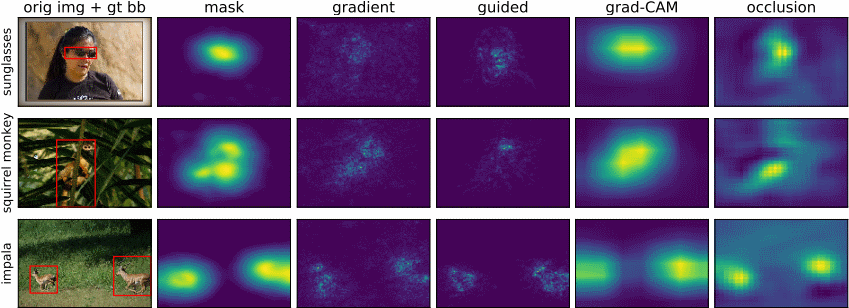
\includegraphics[scale=0.65]{perturb.png}
\caption{(Adapted from \cite{perturb_fong}) Comparison of methods discussed so far: Mask generation \cite{perturb_fong}, Gradient (saliency maps) \cite{saliencyII}, Guided Backpropagation \cite{springenberg}, Grad-CAM \cite{gradcam} and Occlusion \cite{zeilerfergus2013}. Ground truth bounding boxes are labelled ``gt bb''.}
\label{comparisonimg}
\end{figure}

%occlusion and ablation

%occlusion mask, zeiler and fergus

%Understanding Deep Networks via Extremal Perturbations and Smooth Masks
%https://arxiv.org/abs/1910.08485

%Interpretable Explanations of Black Boxes by Meaningful Perturbation
%http://openaccess.thecvf.com/content_ICCV_2017/papers/Fong_Interpretable_Explanations_of_ICCV_2017_paper.pdf


For completeness, some NN methods which do not attribute the contribution of input features specifically (or project internal model signals onto the input space) are not within project scope as a result, but are mentioned here. These are `concept vector' methods that extract model behaviour across layers: Net2Vec \cite{net2vec} and Testing with Concept Activation Vectors (TCAV) \cite{tcav}.

% \footnote{For the reader's interest, these were developed almost simultaneously from rival labs at Oxford and Google.}.




\section{Model-Agnostic Methods} \label{sec:modelag}

In parallel to the literature aimed at explaining neural network model behaviour, a standalone approach in the interpretability literature is to find model-agnostic explanations. Similar to the motivation for perturbation-based methods (and with overlap), these are `black-box' methods that make no restrictive assumptions about model architecture or classification task at all, and therefore can theoretically be applied to any model or task. Stark differences in approach and computational complexity still exist however. The most prominent methods in this sub-field are listed below.


\subsection{Perturbation-Based} \label{sec:perturbag}
Described in Section \ref{sec:otherms}, perturbing the input space (by toggling feature patches) is one way to isolate model behaviour. Changes in output score reveal importance in the occluded inputs. Several methods implement this intuition by training ``surrogate'', interpretable models around the isolated features that are locally relevant to a single prediction. These include Local Interpretable Model-Agnostic Explanations (LIME) \cite{lime}, Anchors \cite{anchors} and similar variants \cite{local}.

\subsubsection{LIME}
LIME's authors propose that non-linear, complex decision boundaries can be approximated locally around a single prediction via a simpler model that only relies only on the ``neighbourhood'' of the relevant input space \cite{lime}. 

\begin{figure}[h]
\centering
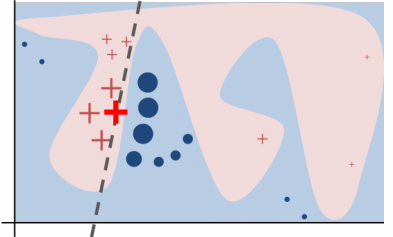
\includegraphics[scale=0.65]{lime_figure.png}
\caption{(From \cite{lime}) LIME's intuition about complex decision boundaries.}
\label{limeimg}
\end{figure}

To compute explanations, LIME trains an interpretable model (i.e. decision tree or Lasso regression) on permuted samples from a given instance, weighted by their proximity to the instance being explained. The training simply minimises mean-squared error based on the samples' black-box predictions. Finally, the interpretable model's weights on these proximal features (superpixels in the case of image data) represent the `explanation' for the underlying instance. 

The formulation in the paper is relatively vague however, particularly with regards to the size of the region of influence / neighbourhood that should be used for finding relevant features. The vagueness was potentially motivated by their intention to be agnostic about the choice of explanation model and the black-box model, though this leaves questions about the accuracy-interpretability compromise largely unaddressed. Generating samples and training models for each sample is also extremely performance costly. Even for a confident prediction and using many samples, instability from random sampling makes an explanation undesirably non-deterministic. This was noted by the authors \cite{lime}. The authors of the mask generation technique described in Section 1.3.3 note that LIME bears similarity to their perturbation approach, but takes significantly longer to converge and produces a coarser heatmap via super-pixels instead of their pixel-level attribution \cite{perturb_fong}.

Despite these shortcomings, LIME's simplicity and complete compatibility across all model families and classification tasks explains its high popularity among model-agnostic methods.

\subsubsection{Anchors}

LIME's problems motivated a more recent successor called ``Anchors: High-Precision Model-Agnostic Explanations'' by its original authors \cite{anchors}. They replaced the use of simple local models with high fidelity if-then rules around a prediction, and give a framework for finding those rules efficiently. A rule (termed an `anchor' explanation) is one that, ``[...] sufficiently anchors an explanation locally, such that changes to the rest of the features of the instance do not matter'' \cite{anchors}. 

Formal ways to define the optimal region of influence (`coverage'), build rule accuracy (`precision'), and calculate rules efficiently were devised - three key improvements over their LIME proposal.

Though these anchor rules are highly interpretable, code available from the authors is limited and (possibly as a result) it has less popularity both in practice and in the literature. The GitHub repository provides for example a rough implementation for only text and tabular data and not image data \cite{anchorsrepo}.

\subsection{Other Model-Agnostic Methods} \label{sec:othermodelag}

\subsubsection{SHAP Framework} 

Many methods have been listed so far and a reader may be fatigued of the variety. The SHAP framework (SHapley Additive exPlanations) by Lundberg \& Lee (2017) was a push-back on this issue of method proliferation, showing links between many existing methods with a theoretical approach from game theory \cite{shap}. It has become extremely popular among researchers from all sub-fields in interpretability due to its attractive formal properties and `outsider' formulation, as well as its implementation approximations for many model families and a well-maintained GitHub repository to host those implementations\footnote{The SHAP paper has over 1000 citations and its GitHub has over 9000 `stars' at the time of writing \cite{shaprepo}, despite only being published in late 2017.}.
 
The game theoretic concept of Shapley values are a unique solution to the problem of calculating fair, marginal per-player rewards for the reward earned collectively in a cooperative game \cite{shapley}. Since each player's contribution may produce interaction effects with others, they are calculated by averaging contributions in all possible sub-coalitions of players. In the context of machine learning, if features are taken as players, the method can be applied to a prediction (the ``payoff'') and it retains its per-player theoretical properties. These qualities include \textit{efficiency}, which is that the sum of \textit{p} constituent input feature contributions (Shapley value $\phi_{j}$ for a feature \textit{j}) must equal the difference between a prediction of an input \textit{x} ($\widehat{f}_{x})$ and an average for all inputs (an `expectation' of model output $E_X(\widehat{f}(X))$):
\begin{align}
\sum_{j=1}^{p}\phi_{j} = \widehat{f}_{x} - E_X(\widehat{f}(X))
\end{align}

A key problem is that finding $\phi_{j}$ requires iteratively computing outputs for all feature subsets including \textit{j} and is therefore computationally infeasible for large input spaces\footnote{They are however commonly used in low-dimensional linear regression settings, like in economics for example, for calculating global feature importances when features are dependent \cite{shapley}.}.

SHAP values are an implementable version of Shapley values. They connect Shapley value theory with local explanation techniques including LIME and DeepLIFT \cite{shap}.  They are formulated as the difference between expected model output (approximated by an average background data sample's prediction) and the instance at hand being predicted. The authors show that the game theoretical properties including efficiency apply to a whole class of `additive feature attribution methods', both model-specific (e.g. DeepLIFT) and model-agnostic. They provide several model-specific approximations for implementing their attributions, one based on Integrated Gradients and another based on DeepLIFT.

% MISSING CRITICAL EVALUATION: Discuss furter in below section??
 %note a similarity between LIME and SHAP: 
 
 
%\subsubsection{Explanation Vectors} 
%Finally, an older model-agnostic method briefly mentionable is Explanation Vectors, by Baehrens et al. (2010)  \cite{explvectors}. 


\section{Evaluation of Attribution Methods}

Creators of feature attribution methods tend to provide visual comparisons with existing methods, as for example in Figure \ref{comparisonimg}. An issue is that qualitative evaluation is often left to the reader, who is encouraged to infer the author's saliency maps are either equal in standing or more aesthetically pleasing than another method's.

Lack of evaluation \textit{independent} of method creators is another issue. Introduced methods do often suggest their own interpretability criteria, though with little reference to criteria in the prior art, and so the interpretability field's agreement on desirable standards for interpretability is low. To some extent, the proliferation in attribution methods (mostly variants) can be attributed to these unfortunately subjective and still actively researched desiderata.

There have however been efforts to unify existing methods. SHAP's momentum in the literature can somewhat be explained by its ability to show how existing methods are related and that it demonstrates where one can be preferable. This research section therefore aims to:

\begin{enumerate}

\item Overview attempts like SHAP that have independently evaluated methods and performed `unification' or comparison studies;
\item Examine existing evaluation criteria that method authors have independently proposed, and;
\item Describe existing software for generating explanations, that package several methods for visual comparison for use by researchers and practitioners.

\end{enumerate}

\subsection{Existing Studies} \label{sec:existing_studies}
\subsubsection{Towards a Rigorous Science of Interpretable Machine Learning \cite{paradigms}}

Doshi-Velez \& Kim (2017) provided an influential set of guidelines or ``evaluation paradigms'' for evaluating interpretability techniques, arranged in three levels of increasing abstraction \cite{paradigms}. This motivation was to provide a scientific basis for the different objectives in evaluation that method authors implicitly target (both qualitative and quantitative):

\begin{enumerate}
\item \textbf{Functionally-grounded}: How well the attribution method performs on quantitative criteria: `proxy' metrics for explainability like weakly supervised object localisation (Section X).
\item \textbf{Human-grounded}: How much everyday people agree that an explanation is visually superior to another: user studies as an example.
\item \textbf{Application-grounded}: How well the explanation helps domain experts solve real tasks; such as a radiologist agreeing with fractures pointed out by a model trained on X-ray data.

\end{enumerate}

Research on evaluation criteria below (Section \ref{sec:existing_criteria}) has focused on functionally-grounded criteria, since these are more common in the literature and since higher-level paradigms are difficult to compare objectively.

\subsubsection{Towards Better Understanding of Gradient-based Attribution Methods \cite{ancona}}
Similar to SHAP in motivation, an independent attempt at providing a unified framework for the gradient-based class\footnote{The authors do not distinguish between backpropagation and gradient-based methods.} of attribution methods was provided by Ancona et al. (2017) \cite{ancona}. In their work they prove conditions of equivalence between Layerwise Relevance Propagation and Gradient * Input, and DeepLIFT and Integrated Gradients (Section \ref{sec:modelspec}). Another major contribution was to propose a generalisation for the ideal `additivity' property that SHAP's authors noted defined a class of methods (Section \ref{sec:othermodelag})\footnote{The authors actually reference the properties of \textit{Completeness} (proposed by the authors of Integrated Gradients \cite{integrated}) and \textit{Summation to Delta} (proposed by the authors of DeepLIFT \cite{deeplift}), two variants of a similar idea to additivity.}. This criteria was termed \textit{Sensitivity-n}: ``[...] when the sum of the attributions for any subset of features of cardinality \textit{n} is equal to the variation of the output $S_{C}$ caused by removing the features in the subset'' \cite{ancona}.

Some of their key insights were that existing methods like DeepLIFT and Integrated Gradients show very high correlation, that the former therefore acts as an approximation of the latter in practice, and that on complex model architectures like InceptionV3, all gradient-based methods produce noisier saliency maps and less appealing explanations.

\subsubsection{Sanity Checks for Saliency Maps \cite{sanity}}


% theoreticla contributions are scarce
% https://arxiv.org/pdf/1705.05598.pdf


This paper by Adebayo et al. (2018), along with Lundberg \& Lee (2017) (SHAP's authors) and Ancona et al. (2017) above, have been the three main independent contributions towards understanding and unifying the model-specific set of feature attribution methods described in earlier sections of this chapter. This motivation was similar though more practical than theoretical: find an actionable methodology to help a practitioner / researcher decide between competing attribution methods.

\begin{figure}[h]
\centering
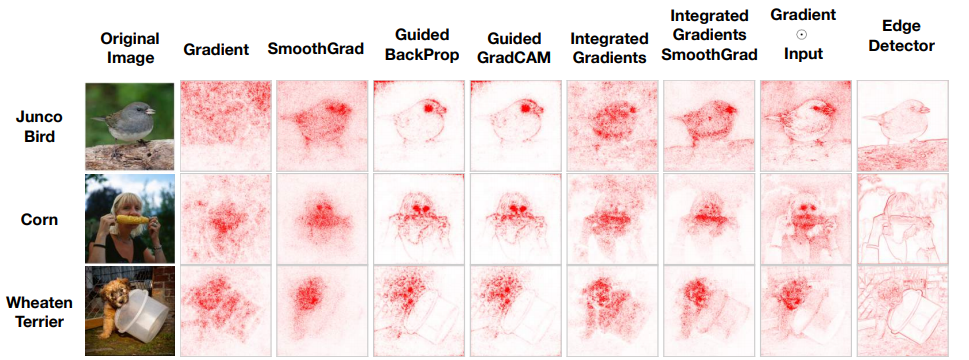
\includegraphics[scale=0.55]{adebayo_panel.png}
\caption{(From \cite{sanity}) The panel of methods examined by Adebayo et al. (2018), all previously discussed in Section \ref{sec:modelspec}. They highlight that an edge detector alone can produce a mask similar to the output of some methods.}
\label{adebayoimg}
\end{figure}


The methodology proposed was a set of two statistical randomisation tests (`sanity checks'):

\begin{enumerate}
\item \textbf{Model Parameter Randomisation Test:} A misleading attribution method could be insensitive to model parameters, so an untrained version of the same model with random weights should not produce a similar saliency map.
\item \textbf{Data Randomisation Test:} A misleading method could be dependent on training labels: a test with randomly permuted labels should therefore show significantly different saliency maps.
\end{enumerate}

For comparisons between a normal attribution output and a modified one according to one of those two experiment conditions, the authors use similarity metrics including Spearman rank correlation and a structural similarity (SSIM) index. Note these metrics do not evaluate one method's similarity with another: only the similarity with its modified version. Some insights are prepared from these metrics, like that Guided Backpropagation and Gradient * Input show unexpected insensitivity (perform badly on the sanity checks). 

% based alone on visual inspection of an input image multiplied with an edge detector's output. The conclusion was 

One problematic point they emphasise though is that non-performing saliency methods may only be visually salient because they act like an edge detector (Figure \ref{adebayoimg}). Although the work valuably points out that observers might have confirmation bias when viewing highlighted edges in a saliency map, this qualitative conclusion ignores the role of connected regions and pixel-wise attribution intensities, which some methods may have as a strength over others. These latter two criteria are arguably as important or more important for visual quality than edges alone, and the authors' similarity metric results also do not relate to the standalone observation about edges.

%Evaluating neural network explanation methods using hybrid documents
% https://arxiv.org/pdf/1801.06422.pdf

% robustness
% https://arxiv.org/abs/1806.08049

% SHAP
% "The thread of unity that SHAP weaves through the literature is an encouraging sign that common principles about model interpretation can inform the development of future methods."

\subsection{Existing Criteria} \label{sec:existing_criteria}

% Table: Sensitivity-N, Implementation Invariance


% sundarajan et al. (2017

\subsubsection{Saliency Metrics (Quantitative Approach)}

Some method authors however have made an effort to account for regions in method evaluation. In particular, `weakly supervised object localisation' (WSOL) has been the technique used for evaluating saliency maps via bounding boxes derived from a segmentation algorithm (in natural image classification settings). It was first applied by Simonyan et al. (2014) while introducing the original saliency maps method (Section \ref{sec:gradient}) \cite{saliencyII} . Those authors used a colour segmentation algorithm on thresholded saliency maps, found bounding boxes on the segmented regions, and then submitted their annotations to an ILSVRC-2103 localisation challenge where they out-performed many fully supervised algorithms. 

The paper that introduced CAM saliency maps (Section \ref{sec:gradient}, \cite{cam}) used a similar technique and has been considered the seminal work for use of WSOL \cite{choe}. They chose a 20\% quantile threshold for CAM values before finding the largest connected component in each map. Unlike Simonyan et al. who only evaluated via the competition, CAM's authors independently evaluate their derived bounding boxes using an intersection-over-union metric (thresholded at 0.5 to exclude instances where the method was significantly off). Their results on an ILSVRC validation set outperformed the benchmarks of localisation-trained models.

\begin{figure}[h]
\centering
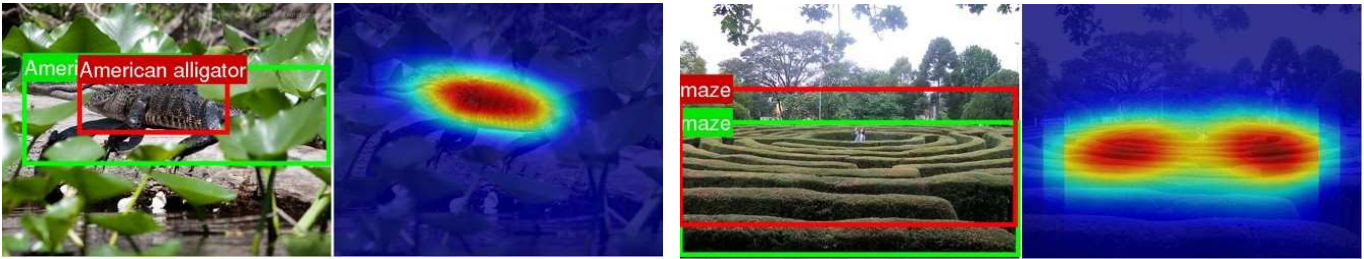
\includegraphics[scale=0.4]{iou_litreview.png}
\caption{(Adapted from \cite{cam}) CAM's predicted bounding box in green and the ground truth annotation in red  (left in each sub-pane), and the original CAM (right in each sub-pane). Their IOU metric is calculated over the annotations.}
\label{adebayoimg}
\end{figure}

Notably this IOU metric does not account for the weight of the attribution in any one pixel, which is relevant to most methods. The methodology also unfairly penalises more perforated-looking saliency maps due to relying on segmentation algorithms to find connected components and therefore ignoring pixel-level detail. On the one hand, connected components are more observer-friendly explanations of single objects (with an implicit assumption that the underlying model also cares about connected regions), though on the other hand some methods may be noisier and so may be punished harshly for having small, disconnected sub-regions yet still maintaining saliency in the `bigger picture'.

Dabkowski \& Gal (2017) compensate for the latter problem by proposing an augmented localisation metric that takes a bounding box of the \textit{entire} salient region, rather than just a thresholded and single-component subset of the saliency map \cite{dabowski}. A strong aspect of their work was to provide a ``Max box'' baseline in reporting localisation error: this reports the ground truth box's overlap with the whole image. Where the localisation error is similar, this allows them to suggest the interpretability of their generated localisation boxes is similar to the ground truth boxes themselves.

Independently of the explainability literature, pixel-wise mask-based metrics have been developed for generic WSOL applications by Choe et al. (2020)  \cite{choe}, though it seems these have not been applied in the context of evaluating explainability techniques.

\subsubsection{Higher Level Criteria (Qualitative Approach)}

Some authors sidestep the functionally-grounded approach to method evaluation and evaluate on higher level criteria. These proposed desiderata are summarised in Table 1.X, from lower to higher levels of abstraction:

consistency between models
input invariance
transferability
trust
fair and ethical decision making

Across in the model-agnostic camp Ribeiro et al. (2016) have made the case for model flexibility as a strong motivation for explanation technique usability \cite{case_for_model_ag}. When comparing a tree-based model with a deep learning model, for example, neither a practitioner nor a researcher can get a fair idea of interpretability if two explanations are different in representation on account of different attribution methods. The observation by Ancona et al. (2017) that more complex architectures are not explained as well by current model-specific techniques also supports this argument (Section \ref{sec:existing_studies}) \cite{ancona}.

% gradcam paper "What makes a good visual explanation?"

%https://arxiv.org/abs/1907.09701
%https://distill.pub/2020/attribution-baselines/

%https://arxiv.org/pdf/1711.00867.pdf

%sanity checks for saliency maps
%https://arxiv.org/pdf/1810.03292.pdf

%unreliability of saliency methods
%https://arxiv.org/pdf/1711.00867.pdf

%https://medium.com/swlh/breaking-down-the-black-box-39403b0f64a3

%IOU: Network Dissection: Quantifying Interpretability
%https://arxiv.org/abs/1704.05796

%\cite{saliencyII}
%Section 3.2 Weakly Supervised Object Localisation
%weakly supervised object localisation from Saliency Maps
%used a segmentation algorithm and entered their saliency
% map into ILSVRC-2013 localisation challenge

%http://cnnlocalization.csail.mit.edu/Zhou_Learning_Deep_Features_CVPR_2016_paper.pdf
% CAM authors also test CAMs on object localisation without bounding box annotation %"Weakly-supervised object localization"


% implementation invariance and sensitivity (integrated gradients)
% https://arxiv.org/pdf/1703.01365.pdf

% coverage, precision and effort from a-LIME
% https://arxiv.org/pdf/1611.05817.pdf


\subsection{Existing Explanation Frameworks}

Ancona et al. (2017) developed a software package called \textit{DeepExplainer} to support their unified framework \cite{deepexplainerrepo}. It implements a suite of the methods they showed relationships between: Saliency Maps, Gradient * Input, Integrated Gradients, DeepLIFT and Occlusion (Section \ref{sec:modelspec}). It provides abstraction over these methods with some parameter specification allowed: .

Aimed at practitioners for auditing their models for bias, \textit{FairML} was developed by Adebayo (2017) \cite{fairml}. This package

There are no explanation frameworks for collecting both model-agnostic and model-specific techniques for saliency maps. Additionally, no automated method evaluation frameworks for WSOL-based evaluation are known to be available.

%TreeExplainer repo??

%TensorFlow implementation for SmoothGrad, Grad-CAM, Guided backprop, Integrated Gradients and other saliency techniques  https://github.com/PAIR-code/saliency

%Skater - a unified framework for model-agnostic interpretation --> global and local
%DeepExplainer

%TorchRay https://github.com/facebookresearch/TorchRay

% Innvestigate package, used for DeepLIFT (Section X)

% https://openreview.net/forum?id=Sy21R9JAW
% pytorch
% deepexplainer


\end{document}
